%%
%%  Department of Electrical, Electronic and Computer Engineering.
%%  EPR400/2 Final Report - Section 4.
%%  Copyright (C) 2011-2021 University of Pretoria.
%%

\section{Results}

\subsection{Summary of results achieved}
\begin{table}[H]
  \centering
  \begin{tabularx}{\textwidth}{|X|X|l|}
    \hline
    \textbf{Intended outcome}                                                                                                                                                    &
    \textbf{Actual outcome}                                                                                                                                                      &
    \textbf{Location in report}                                                                                                                                                                                                                                                                                                                  \\
    \hline
    \multicolumn{3}{|l|}{\textbf{Core mission requirements and specifications}}                                                                                                                                                                                                                                                                  \\
    \hline
    The system must track mosquitoes in a mosquito enclosure and illuminate a mosquito every 5 seconds.                                                                          &
    The system tracks mosquitoes in the enclosure and illuminates a mosquito when it is stationary or moves predictably.                                                         &
    \autoref{sec:results_tracking}                                                                                                                                                                                                                                                                                                               \\
    \hline
    The laser must be able to illuminate a set point within 2 seconds accurate to within 1 millimetre.                                                                           &
    Yes                                                                                                                                                                          &
    sec                                                                                                                                                                                                                                                                                                                                          \\
    \hline
    The system must be able to detect mosquitoes with a 90\% accuracy and 5\% false positive rate. The detection must be updated at least every 500 milliseconds.                & Weet nie. The detection is updated every 500 milliseconds.                                                                                              & sec \\
    \hline
    The system must be able to track mosquitoes with 90\% accuracy of correct association between frames after 5 seconds.                                                        & Weet nie.                                                                                                                                               & sec \\
    \hline
    \multicolumn{3}{|l|}{\textbf{Field condition requirements and specifications}}                                                                                                                                                                                                                                                               \\
    \hline
    Mosquitoes should be in an enclosure with controlled lighting and white lining on all the sides except the front facing side. The enclosure should be at least 1 metre wide. & The enclosure has \glspl{led} to control the lighting and white lining on all the sides except the front facing side. The enclosure is 0.9 metres wide. & sec \\
    \hline
    If mosquitoes cannot be obtained a suitable substitute will be used. The substitute will be a similar flying insect.                                                         & Mosquitoes and similar flying insects were obtained. Dead mosquitoes were also used.                                                                    & sec \\
    \hline
  \end{tabularx}
  \caption{Summary of results achieved.}
  \label{tab:results_summary}
\end{table}

\subsection{Qualification tests}
\textbf{Qualification test 1: Test of tracking and illuminating a mosquito}\\

\textit{Objectives of the test or experiment}\\
The objective of this experiment is to determine whether the system can track and illuminate a mosquito in the mosquito enclosure. The requirement states that the system must track mosquitoes in the enclosure and illuminate a mosquito every 5 seconds.

\textit{Equipment used}\\
The Nvidia Jetson Nano was used as the embedded platform to control the system. The Raspberry Pi Camera Module V2 was used to capture the video feed. The laser turret was used to position the laser. The Nvidia Jetson Nano was connected to user peripherals for user input and output.

\textit{Test setup and experimental parameters}\\
Mosquitoes were simulated with a small black dot attached to a white stick. The stick was inserted into the controller and moved around.

\textit{Results or measurements}\\
\begin{figure}[h]
  \centering
  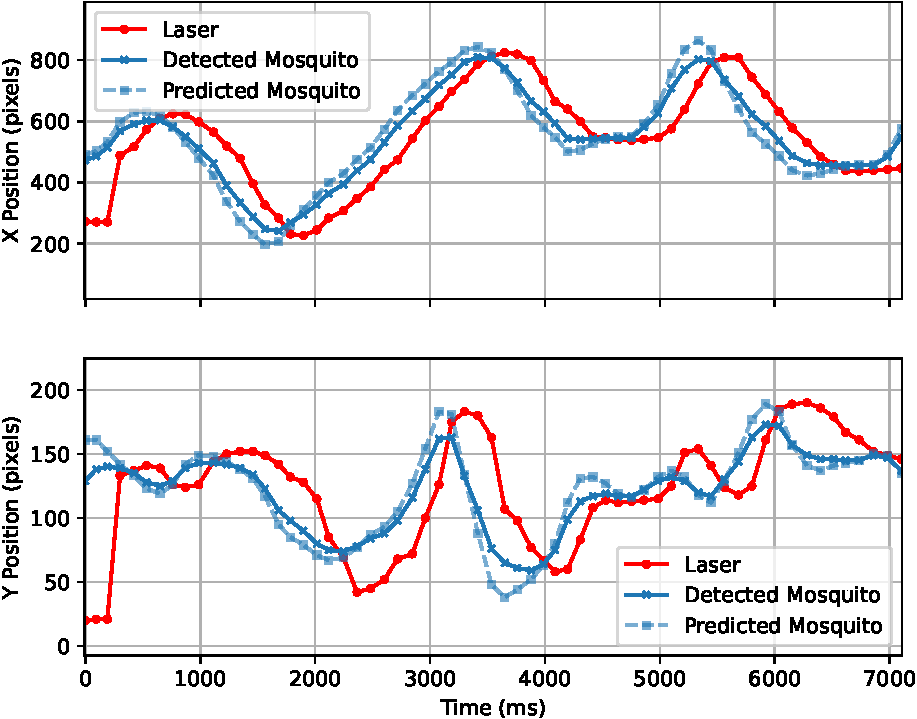
\includegraphics[width=\textwidth]{figures/results/q1_1mos_detection_5fps.pdf}
  \caption{q1 1mos detection 5fps}
  \label{fig:q1_1mos_detection_5fps}
\end{figure}

\begin{figure}[h]
  \centering
  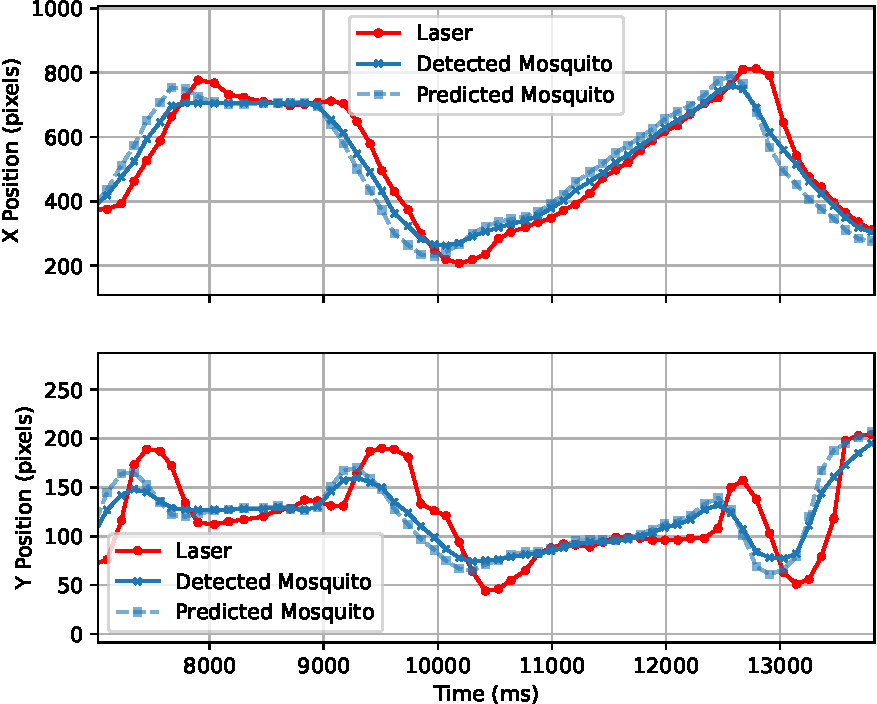
\includegraphics[width=\textwidth]{figures/results/q1_1mos_prediction_5fps.pdf}
  \caption{q1 1mos prediction 5fps}
  \label{fig:q1_1mos_prediction_5fps}
\end{figure}

\textit{Observations}\\

\textbf{Qualification test 2: Measurement of the time taken for the laser to reach a set point}\\

\textit{Objectives of the test or experiment}\\
The objective of this experiment is to measure the time it takes for the laser to reach a set point. The requirement states that the laser must be able to illuminate a set point within 2 seconds accurate to within 1 millimetre.

\textit{Equipment used}\\
The Nvidia Jetson Nano was used as the embedded platform to control the system. The Raspberry Pi Camera Module V2 was used to capture the video feed. The laser turret was used to position the laser. The Nvidia Jetson Nano was connected to user peripherals for user input and output.

\textit{Test setup and experimental parameters}\\
Multiple iterations was performed. The experiment will be performed using both a single step input and a step input with a ramp.

\textit{For a few runs align the set point with a circle or square with radius of 1mm and take a picture of the laser setting point to see if it is accurate to 1mm. Also measure the amout of pixels for 1mm at a few points then this can be used for the rest of the results.}

\begin{enumerate}
  \item The laser is manually positioned in an arbitrary location in the mosquito enclosure.
  \item The set point is set to an arbitrary location in the mosquito enclosure.
  \item The system is set to set the set point with either a step input or a ramp function.
  \item The turret is started.
  \item The time and position of the laser is recorded for each frame captured by the system until the laser reaches a settling point.
  \item The results are saved, and the experiment is repeated.
\end{enumerate}

\textit{Results or measurements}\\
\begin{figure}[h]
  \centering
  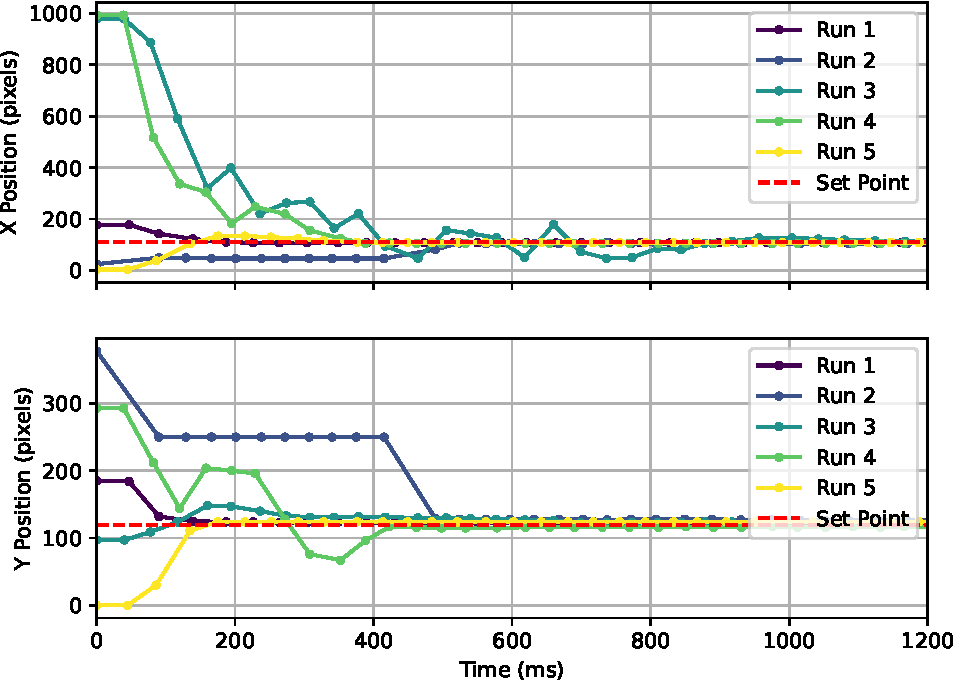
\includegraphics[width=\textwidth]{figures/results/q2.pdf}
  \caption{q2}
  \label{fig:q2}
\end{figure}

\textit{Observations}\\

\textbf{Qualification test 3: Test of mosquito detection}\\

\textit{Objectives of the test or experiment}\\
The objective of this experiment is to determine whether the system can detect mosquitoes in the mosquito enclosure. The requirement states that the system must be able to detect mosquitoes with a 90\% accuracy and 5\% false positive rate. The detection must be updated at least every 500 milliseconds.

\textit{Equipment used}\\
The Nvidia Jetson Nano was used as the embedded platform to control the system. The Raspberry Pi Camera Module V2 was used to capture the video feed. The Nvidia Jetson Nano was connected to user peripherals for user input and output.

\textit{Test setup and experimental parameters}\\
Keep the mosquitoes in the tank constant and vary the threshold for detection and plot the accuracy and false positive rate against the threshold. Either two plots or one plot with two y-axes or a 3d plot.

Create a function that takes in the known number of mosquitoes in the enclosure and saves this, the threshold, and the number of mosquitoes detected for each frame in a file. The first line must be the known num mossies and threshold. The second line must be the number of mosquitoes detected for each frame seperated by commas. The function must also save the average frame rate. The function must run for 1 min.


To determine the update frequency of the detection the following experiment was performed.
\begin{enumerate}
  \item The mosquito enclosure was populated with a varying amount of mosquitoes.
  \item The system was left to run for x time.
  \item The average frame rate was recorded for the duration of the experiment.
  \item The experiment was repeated for different amounts of mosquitoes in the enclosure and with tracking enabled and disabled.
\end{enumerate}

To determine the accuracy of the detection the following experiment was performed.
\begin{enumerate}
  \item The mosquito enclosure was populated with a varying amount of mosquitoes.
  \item The system was left to run for x time.
  \item The number of mosquitoes detected was recorded for the duration of the experiment.
  \item The experiment was repeated for different amounts of mosquitoes in the enclosure.
\end{enumerate}
Kan ek net dooie muskiete plak in die tenk? Kan ek hulle plak of my stokkies en rotbeweeg? Kan ek net kolle gebruik? As ek regte muskiete vang dan vlieg hulle die heel tyd in hoekies waar my kamera hulle nie kan sien nie of hulle gaan sit still.

\textit{Results or measurements}\\

\textit{Observations}\\

\textbf{Qualification test 4: Test of mosquito tracking}\\

\textit{Objectives of the test or experiment}\\
The objective of this experiment is to determine whether the system can track mosquitoes in the mosquito enclosure. The requirement states that the system must track mosquitoes in the enclosure with 90\% accuracy after 5 seconds.

\textit{Equipment used}\\
The Nvidia Jetson Nano was used as the embedded platform to control the system. The Raspberry Pi Camera Module V2 was used to capture the video feed. The Nvidia Jetson Nano was connected to user peripherals for user input and output.

\textit{Test setup and experimental parameters}\\
Compare number of actual mosquitoes to number of tracked mosquitoes.


Plot predicted position vs actual position.


\textit{Results or measurements}\\

\textit{Observations}\\

\newpage

%% End of File.


